 \hoffset1cm % przesunięcie poziome (przykładowo) o 1cm przeznaczone na oprawę

 \documentclass[11pt]{report}
 
 \usepackage[T1]{fontenc}
 \usepackage[utf8]{inputenc}
 \usepackage{graphicx}
 \usepackage{amsmath,amssymb,amsfonts}
 \usepackage{polski}
 \usepackage[raggedright]{titlesec}
 \usepackage{amsmath}
 \usepackage{amssymb}
 \usepackage{indentfirst}
 \usepackage{listings}
 \usepackage{hyperref}
 \usepackage[backend=biber, bibencoding=utf8, style=ieee, dashed=false, isbn=false, doi=false, sorting=anyvt]{biblatex}
 
 \addbibresource{library.bib}
 \DeclareUnicodeCharacter{229}{ę}
 \DeclareUnicodeCharacter{327}{}
 
 \pagestyle{headings}
 
 \renewcommand{\chaptername}{Rozdział}
 \renewcommand{\contentsname}{Spis treści}
 \renewcommand{\figurename}{Rys.}
 \renewcommand{\tablename}{Tab.}
 \renewcommand{\listfigurename}{Spis rysunków}
 \renewcommand{\listtablename}{Spis tabel}
 \renewcommand{\bibname}{Bibliografia}

\makeatletter
\renewcommand{\l@section}{\@dottedtocline{1}{1.5em}{2.6em}}
\renewcommand{\l@subsection}{\@dottedtocline{2}{4.0em}{3.6em}}
\renewcommand{\l@subsubsection}{\@dottedtocline{3}{7.4em}{4.5em}}
\makeatother


 \begin{document}

 \begin{titlepage}
 \centering

\includegraphics[width=0.8 \textwidth]{fig/AGH.jpg}
 \center{\scshape WYDZIAŁ INFORMATYKI, ELEKTRONIKI\\ I TELEKOMUNIKACJI\\
         Kierunek Informatyka}
 \vspace{0.03\textheight}
 \center{\scshape Michał Patyk}
 \bigskip
 \center{\LARGE\bfseries Analiza danych i wzorców dotyczących wydarzeń politycznych na podstawie informacji zgromadzonych w projekcie GDELT}
 \center{(pracownia problemowa)}
 \vspace{0.2\textheight}
 \par
 \rightline{Opiekun: dr hab. inż. Koźlak Jarosław}

 \vspace{0.1\textheight}
 \center{Kraków 2020}
 \end{titlepage}


 \tableofcontents


 \chapter{Wstęp}
 
 \section{GDELT}
 GDELT - Global Database of Events, Language, and Tone - to największa, najbardziej wszechstronna i otwarta baza danych jaka powstała. Wczesne poszukiwania prowadzące do stworzenia GDELT zostały opisane przez Philipa Schrodta w dokumencie \cite{Schrodt2010} w styczniu 2010 r. Zbiór danych jest dostępny na stronie Projektu oraz na platformie Google Cloud gdzie można z niego korzystać przez Google BigQuery \cite{BigQuery2014}. GDELT używa kodowania obserwacji konfliktów i mediacji (CAMEO) \cite{GDELTDocumentation} do rejestrowania zdarzeń. W zbiorze znajdują się dane od 1979 roku do dnia dzisiejszego. 

 
 \section{Stan aktualnej wiedzy}
 \subsection{...}
 
 \section{Motywacja}


 \chapter{Cele pracy, zakres pracy, założenia}\label{ch:cele}

 \section{Cele pracy}
 Celem niniejszej pracy jest...

 \section{Zakres pracy}
 Zakres pracy obejmuje...
 
 
 \section{Założenia i wymagania}
 
 \subsection{Wykorzystane narzędzia}
 \begin{enumerate}
 \item[•] język programowania Python
 \item[•] środowisko programistyczne PyCharm 
 \item[•] internetowe interaktywne środowisko obliczeniowe Notebook Jupyter
 \item[•] hurtownia danych Google BigQuery
 \end{enumerate}
 
 \subsection{Założenia}
 W analizie wykorzystany zostanie głównie zbiór danych GDELT 2.0 od początku 2015 roku do kwietnia 2020.
 
 \subsection{Wymagania}

 
 \section{Efekt końcowy}
 Planowanym efektem końcowym pracy będzie...
 
 \section{Dalsze kierunki rozwoju}
 W tej części zostaną opisane możliwe kierunki rozwoju pracy.
 \subsection{Analiza pod kątem COVID-19}
 \subsection{Analiza pod kątem grup etnicznych}
 \subsection{Analiza pod kątem grup religijnych}
 
 
 \chapter{Przegląd istniejących analiz}\label{ch:przeglad}
 \section{•}
  
 \chapter{Wstępna analiza danych}
 \section{Popularność Polski w zbiorze danych GDELT}
 Jako pierwszą analizę wykonano badanie popularności Polski w zbiorze danych GDELT. Na wszystkich trzech wykresach obserwujemy znaczny wzrost ilości zdarzeń w 2015 roku. Może być to związane z uruchomieniem w GDELT automatycznego tłumaczenia artykułów i co za tym idzie zwiększeniem ilości źródeł danych.
 \subsection{Polska jako Aktor 1}
 Wykers \ref{fig:PLactor1} przedstawia popularność Polski jako aktora 1 skumulowaną dla poszczególnych lat. W roku 2016 obserwujemy szczyt popularności na poziomie około 150 tysięcy zdarzeń.
    \begin{figure}[ht]
	\centering
	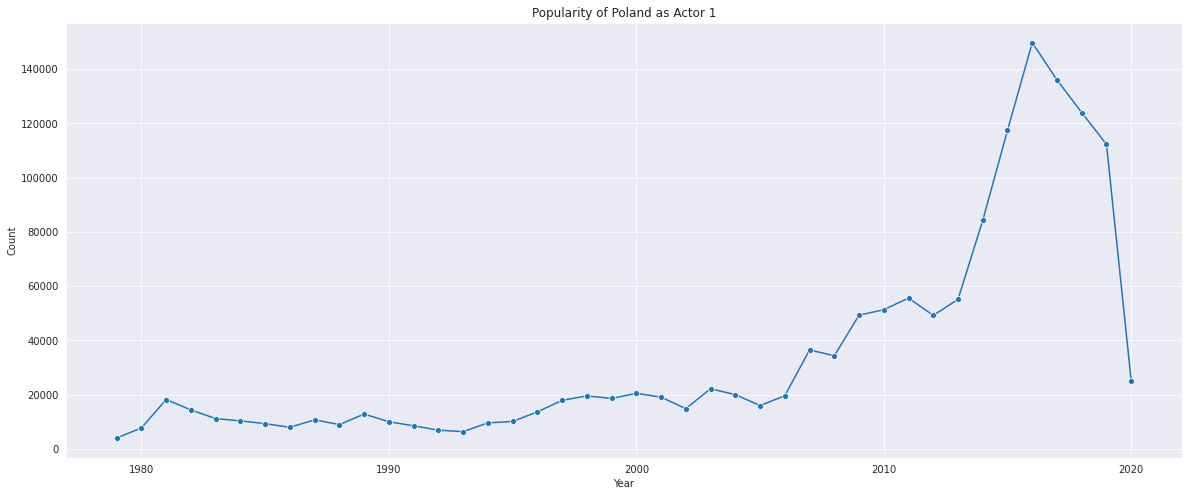
\includegraphics[width=0.8 \textwidth]{fig/PL/PLactor1.png}
	\caption{Ilość zdarzeń z Polską jako aktorem 1. (zródło: opracowanie własne)}
		\label{fig:PLactor1}
	\end{figure}
	
 \subsection{Polska jako Aktor 2}
 Wykers \ref{fig:PLactor2} przedstawia popularność Polski jako aktora 2 skumulowaną dla poszczególnych lat. Kształt wykresu jest bardzo zbliżony do \ref{fig:PLactor1} jednak szczyt popularności jest niższy - na poziomie około 130 tysięcy zdarzeń.
     \begin{figure}[ht]
	\centering
	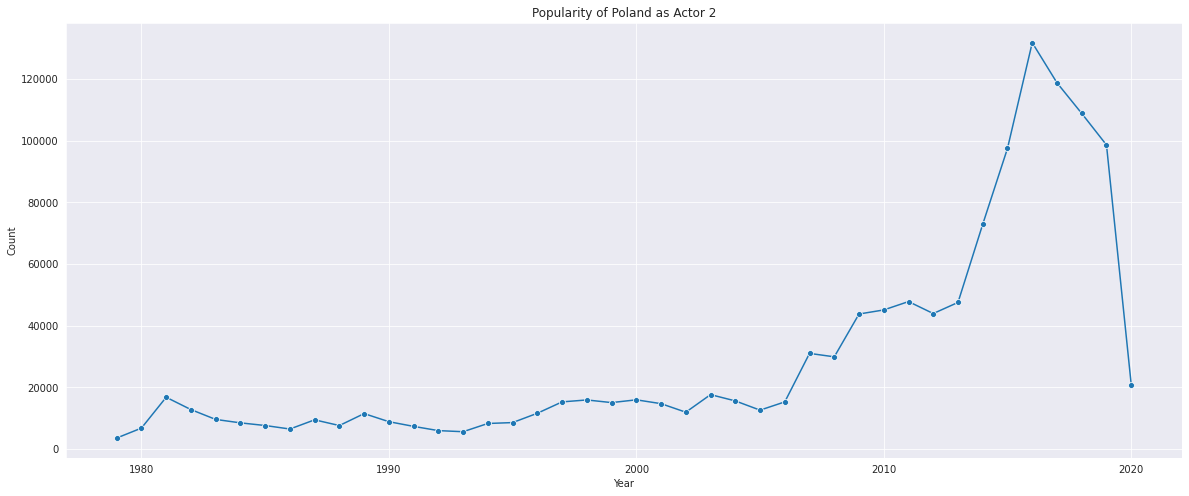
\includegraphics[width=0.8 \textwidth]{fig/PL/PLactor2.png}
	\caption{Ilość zdarzeń z Polską jako aktorem 2. (zródło: opracowanie własne)}
	\label{fig:PLactor2}
	\end{figure}
	
 \subsection{Polska jako miejsce wydarzeń}
 Wykers \ref{fig:PLlocation} przedstawia popularność Polski jako miejsca wydarzeń skumulowaną dla poszczególnych lat. Ponownie kształt wykresu jest zbliżony do \ref{fig:PLactor1}. W tym przypadku szczyt popularności jest wyższy - na poziomie około 210 tysięcy zdarzeń.
     \begin{figure}[ht]
	\centering
	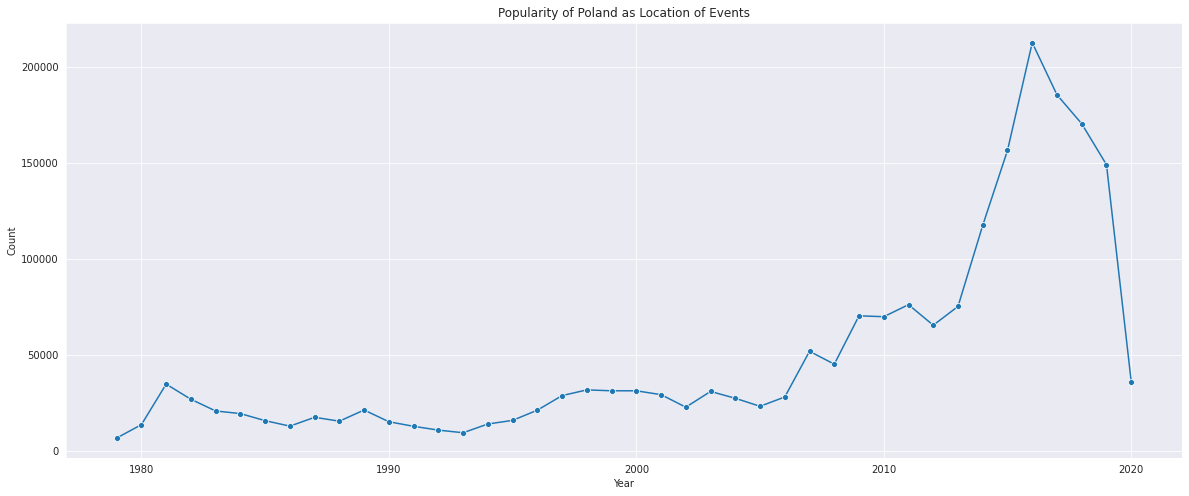
\includegraphics[width=0.8 \textwidth]{fig/PL/PLlocation.png}
	\caption{Ilość zdarzeń z Polską jako lokacją. (zródło: opracowanie własne)}
	\label{fig:PLlocation}
	\end{figure}

 \section{Analiza zbiorcza od 2015 roku}
 \subsection{Kraje jako aktor 1}
 	Wykres \ref{fig:GLOBALactor1} przedstawia sumaryczną ilość zdarzeń od 2015 roku, dla poszczególnych krajów, uszeregowaną malejąco.
      \begin{figure}[ht]
	\centering
	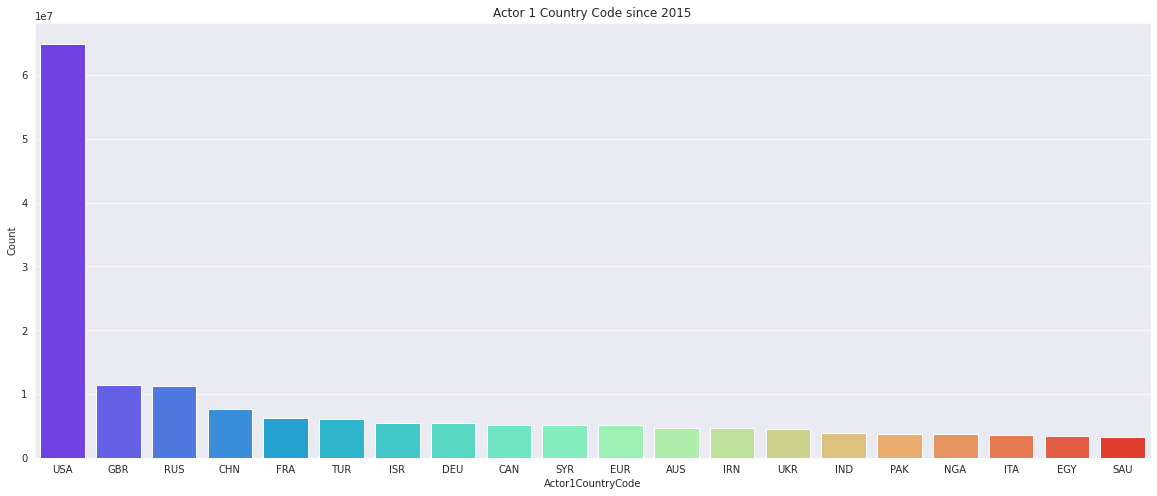
\includegraphics[width=0.8 \textwidth]{fig/GLOBAL/Actor1.png}
	\caption{Ilość zdarzeń dla poszczególnych krajów. (zródło: opracowanie własne)}
	\label{fig:GLOBALactor1}
	\end{figure}
Niekwestionowanym liderem pod względem ilości zdarzeń są Stany Zjednoczone. Dystansują one pozostałe kraje o prawie rząd wielkości.

 \subsection{Ilość zdarzeń w czasie}
 Wykres \ref{fig:GLOBALactor1inTime} przedstawia ilość zdarzeń dla top 5 krajów skumulowaną dla poszczególnych lat.
 WYKRES DO POPRAWY
 	  \begin{figure}[ht]
	\centering
	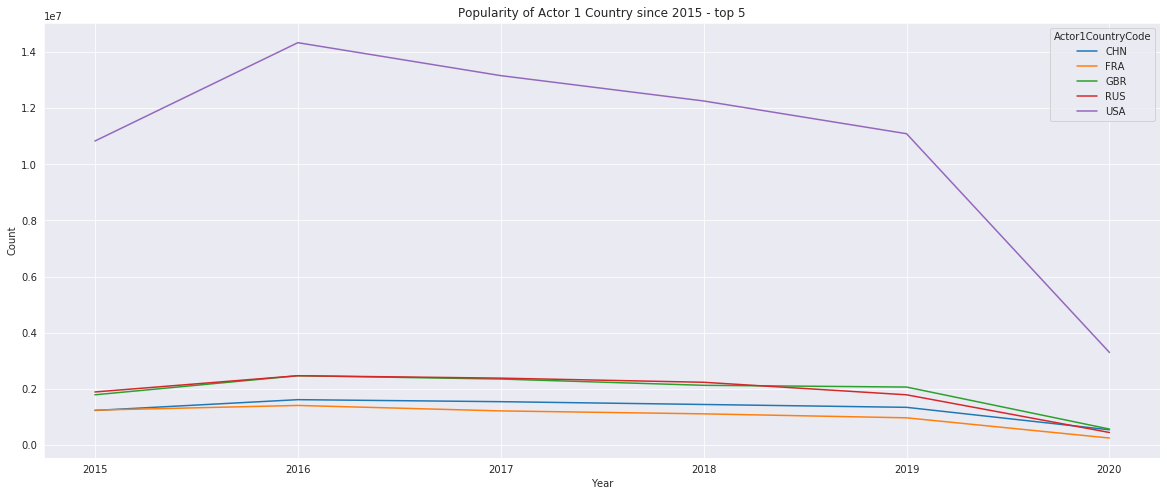
\includegraphics[width=0.8 \textwidth]{fig/GLOBAL/Actor1inTIME.png}
	\caption{Ilość zdarzeń dla poszczególnych krajów w czasie. (zródło: opracowanie własne)}
	\label{fig:GLOBALactor1inTime}
	\end{figure}
 
 \subsection{Popularność bazowych kodów zdarzeń}
  	Wykres \ref{fig:GLOBALEBC} przedstawia sumaryczną ilość zdarzeń od 2015 roku, dla poszczególnych bazowych kodów zdarzeń, uszeregowaną malejąco.
  	  \begin{figure}[ht]
	\centering
	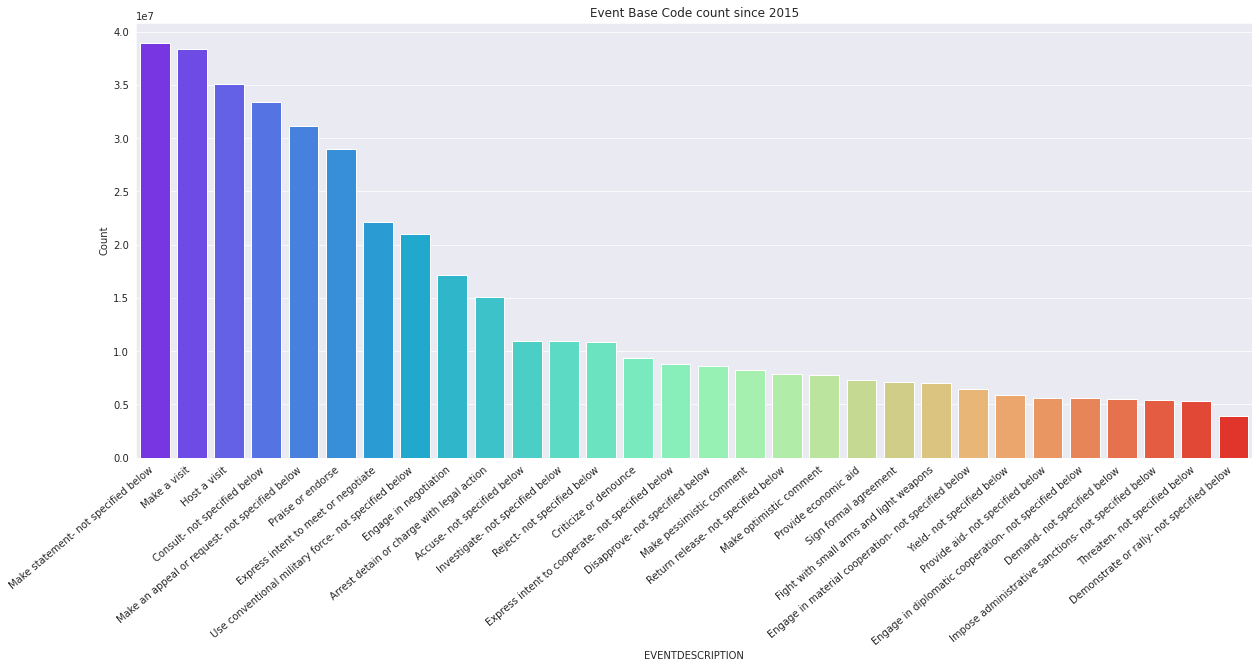
\includegraphics[width=0.8 \textwidth]{fig/GLOBAL/EBC.png}
	\caption{Ilość zdarzeń dla poszczególnych kodów w czasie. (zródło: opracowanie własne)}
	\label{fig:GLOBALEBC}
	\end{figure}
	
 \subsection{Popularność bazowych kodów zdarzeń w czasie}
  Wykres \ref{fig:GLOBALEBCperc} przedstawia ilość zdarzeń dla top 20 bazowych kodów zdarzeń skumulowaną dla poszczególnych lat.
   WYKRES DO POPRAWY
     \begin{figure}[ht]
	\centering
	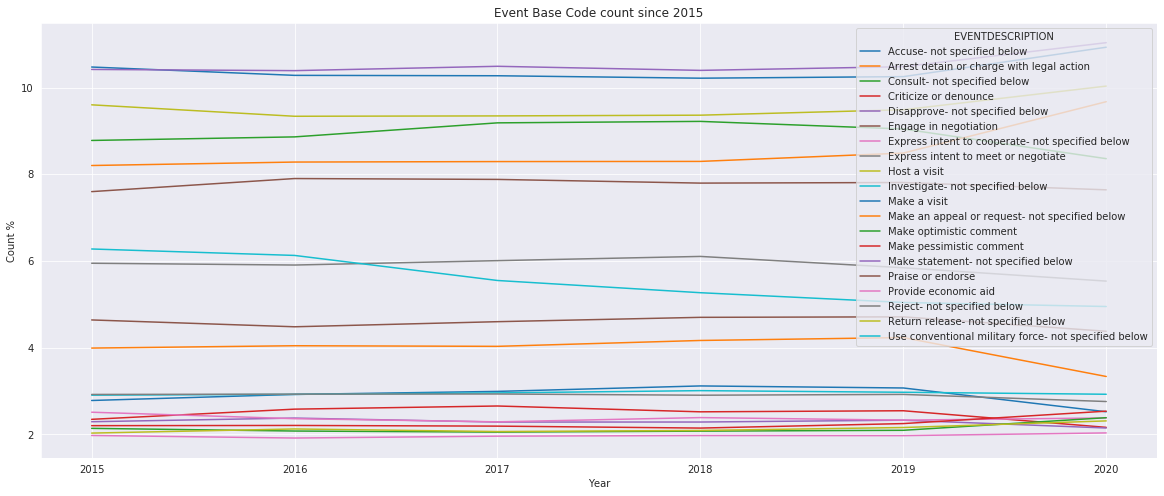
\includegraphics[width=0.8 \textwidth]{fig/GLOBAL/EBCperc.png}
	\caption{Procentowa ilość zdarzeń dla poszczególnych kodów w czasie. (zródło: opracowanie własne)}
	\label{fig:GLOBALEBCperc}
	\end{figure}
	
 \subsection{Popularność podstawowych kodów zdarzeń}
  	Wykres \ref{fig:GLOBALERC} przedstawia sumaryczną ilość zdarzeń od 2015 roku, dla poszczególnych podstawowych kodów zdarzeń, uszeregowaną malejąco.
  	  \begin{figure}[ht]
	\centering
	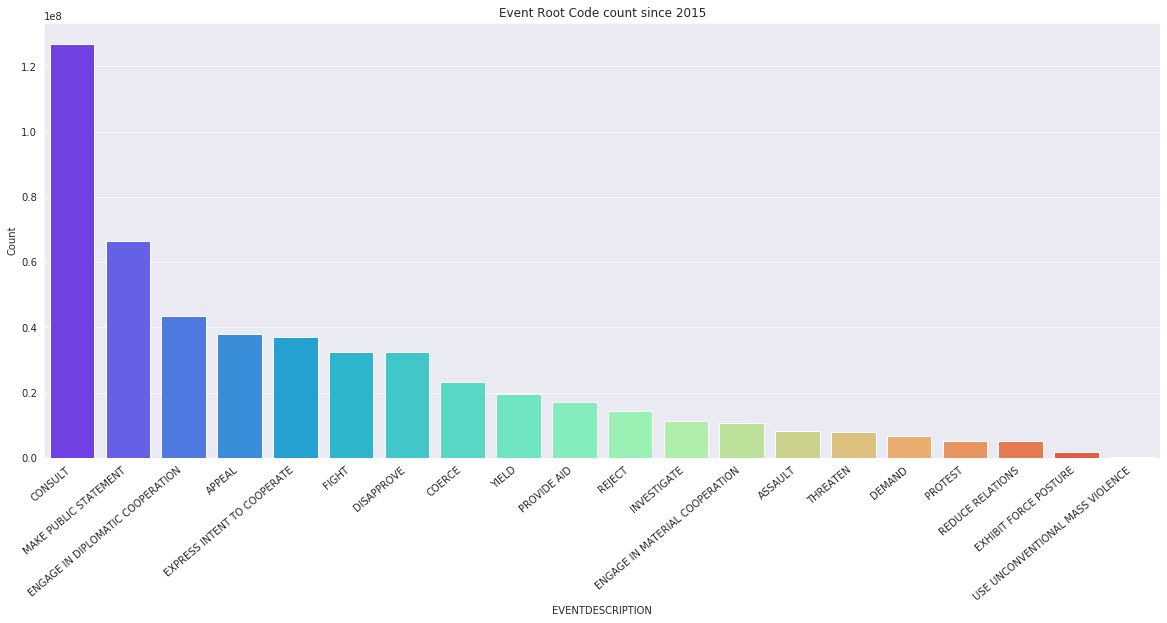
\includegraphics[width=0.8 \textwidth]{fig/GLOBAL/ERC.png}
	\caption{Ilość zdarzeń dla poszczególnych kodów w czasie. (zródło: opracowanie własne)}
	\label{fig:GLOBALERC}
	\end{figure}
	
 \subsection{Popularność podstawowych kodów zdarzeń w czasie}
  Wykres \ref{fig:GLOBALERCperc} przedstawia ilość zdarzeń dla top 20 podstawowych kodów zdarzeń skumulowaną dla poszczególnych lat.
   WYKRES DO POPRAWY
     \begin{figure}[ht]
	\centering
	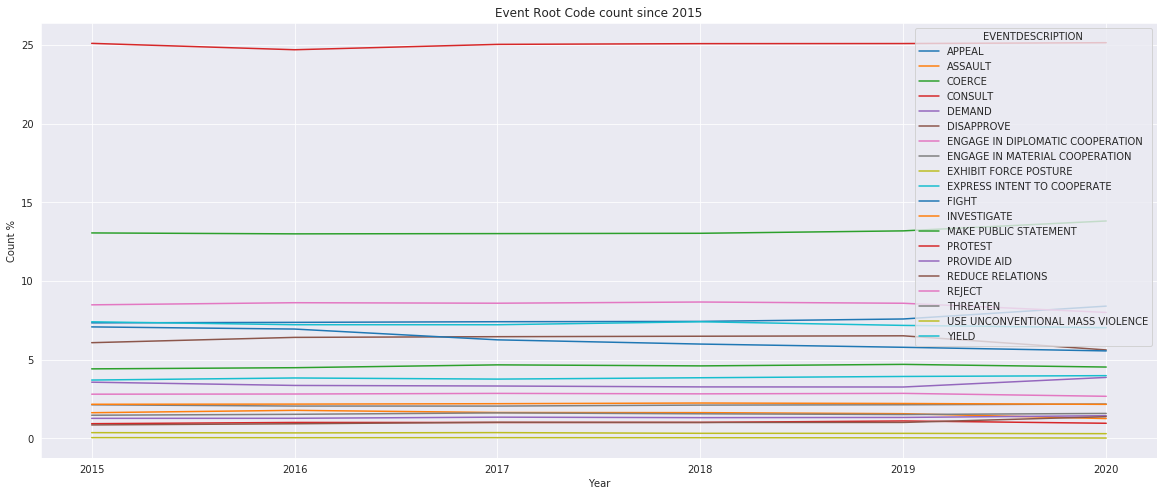
\includegraphics[width=0.8 \textwidth]{fig/GLOBAL/ERCperc.png}
	\caption{Procentowa ilość zdarzeń dla poszczególnych kodów w czasie. (zródło: opracowanie własne)}
	\label{fig:GLOBALERCperc}
	\end{figure}
	
 \subsection{Popularność czterokodów zdarzeń}
  	Wykres \ref{fig:GLOBALQC} przedstawia sumaryczną ilość zdarzeń od 2015 roku, dla poszczególnych czterokodów zdarzeń, uszeregowaną malejąco.
  	\begin{figure}[ht]
	\centering
	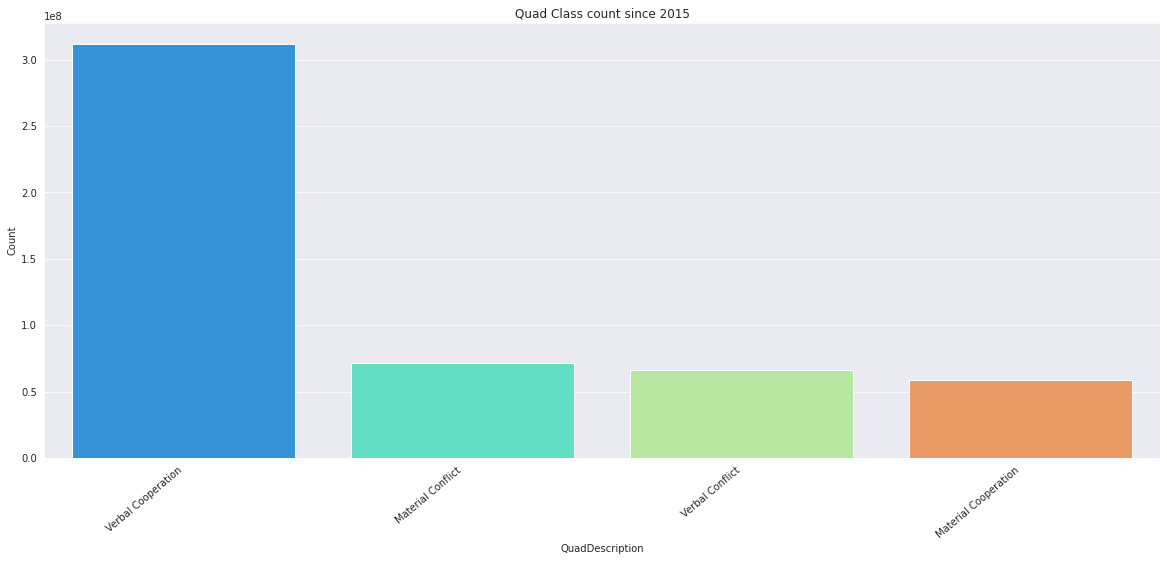
\includegraphics[width=0.8 \textwidth]{fig/GLOBAL/QC.png}
	\caption{Ilość zdarzeń dla poszczególnych kodów w czasie. (zródło: opracowanie własne)}
	\label{fig:GLOBALQC}
	\end{figure}
	
 \subsection{Popularność czterokodów zdarzeń w czasie}
  Wykres \ref{fig:GLOBALQCperc} przedstawia ilość zdarzeń dla czterokodów zdarzeń skumulowaną dla poszczególnych lat.
   WYKRES DO POPRAWY
    \begin{figure}[ht]
	\centering
	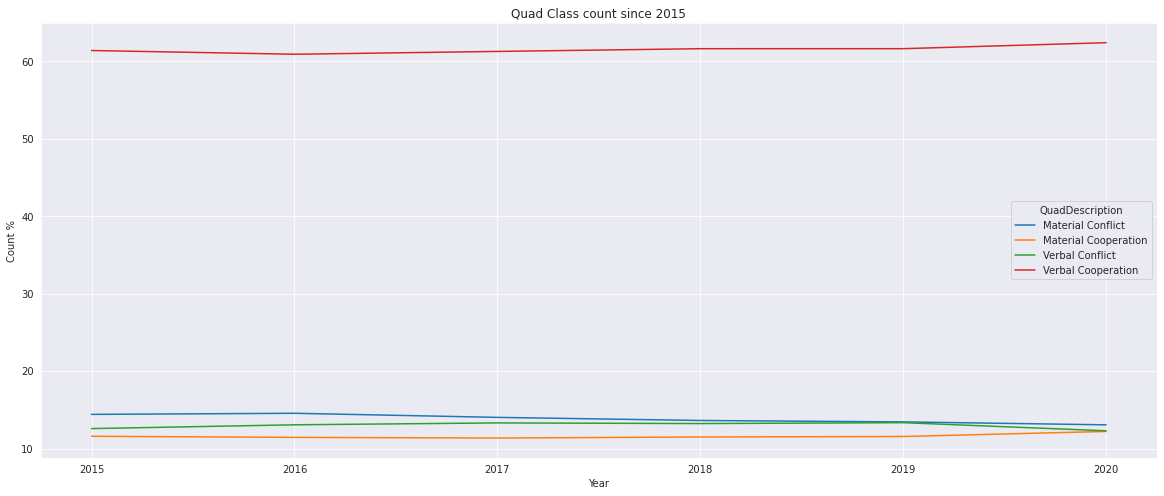
\includegraphics[width=0.8 \textwidth]{fig/GLOBAL/QCperc.png}
	\caption{Procentowa ilość zdarzeń dla poszczególnych kodów w czasie. (zródło: opracowanie własne)}
	\label{fig:GLOBALQCperc}
	\end{figure}

 
 \chapter{Analiza danych dla wybranych krajów}
 \section{Polska}
 
 \subsection{Kraj para do zdarzenia}
    
    \begin{figure}[ht]
	\centering
	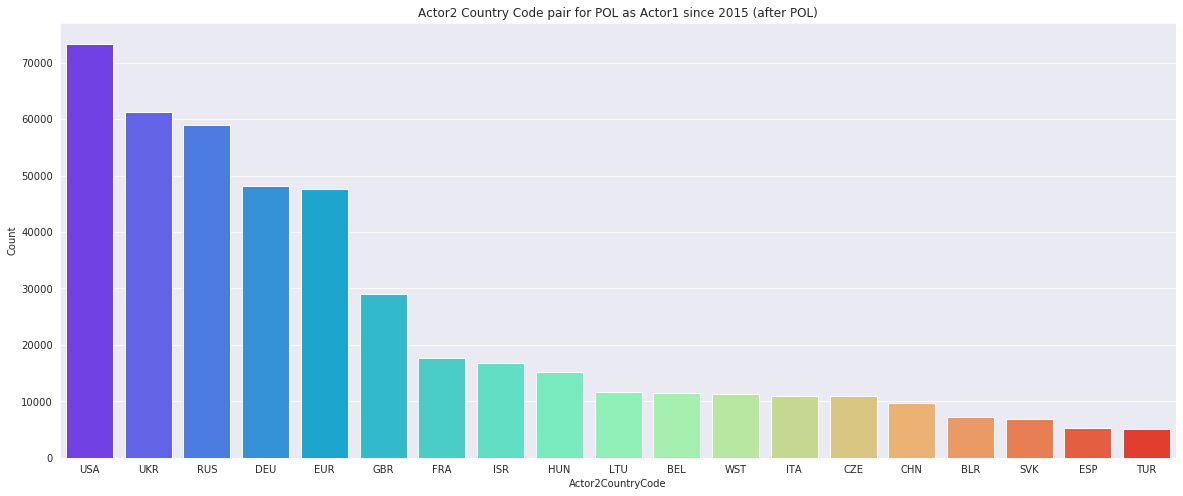
\includegraphics[width=0.8 \textwidth]{fig/PL/PLactor2Pair.png}
	\caption{Ilość zdarzeń w których parą jest dany kraj. (zródło: opracowanie własne)}
	\label{fig:PLpair}
	\end{figure}
	
	   WYKRES DO POPRAWY
	\begin{figure}[ht]
	\centering
	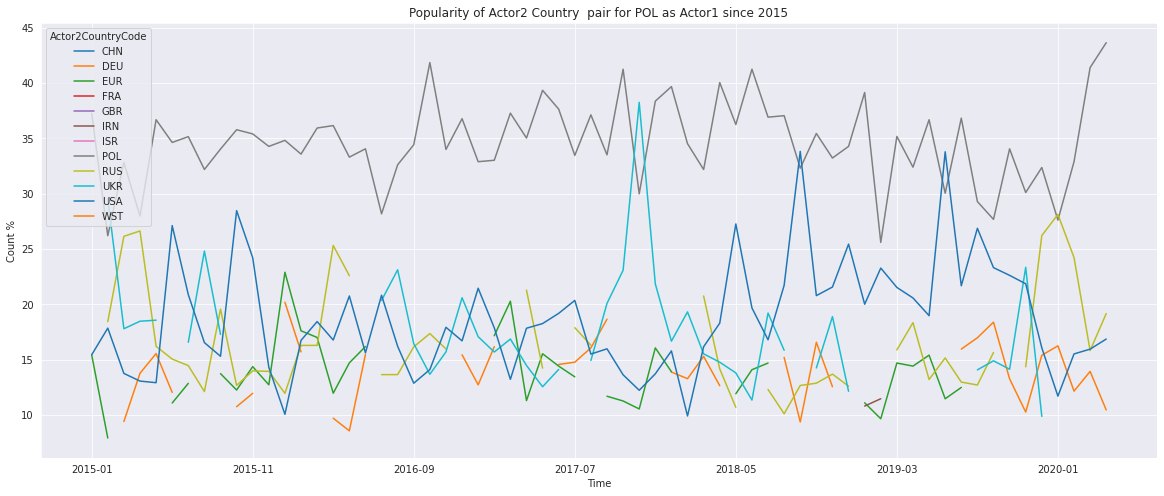
\includegraphics[width=0.8 \textwidth]{fig/PL/PLactor2PairPercinTIME.png}
	\caption{Procentowa ilość zdarzeń w których parą jest dany kraj w czasie. (zródło: opracowanie własne)}
	\label{fig:PLpairPerc}
	\end{figure}
	
 \subsection{Podstawowy kod zdarzeń}
 	
 	\begin{figure}[ht]
	\centering
	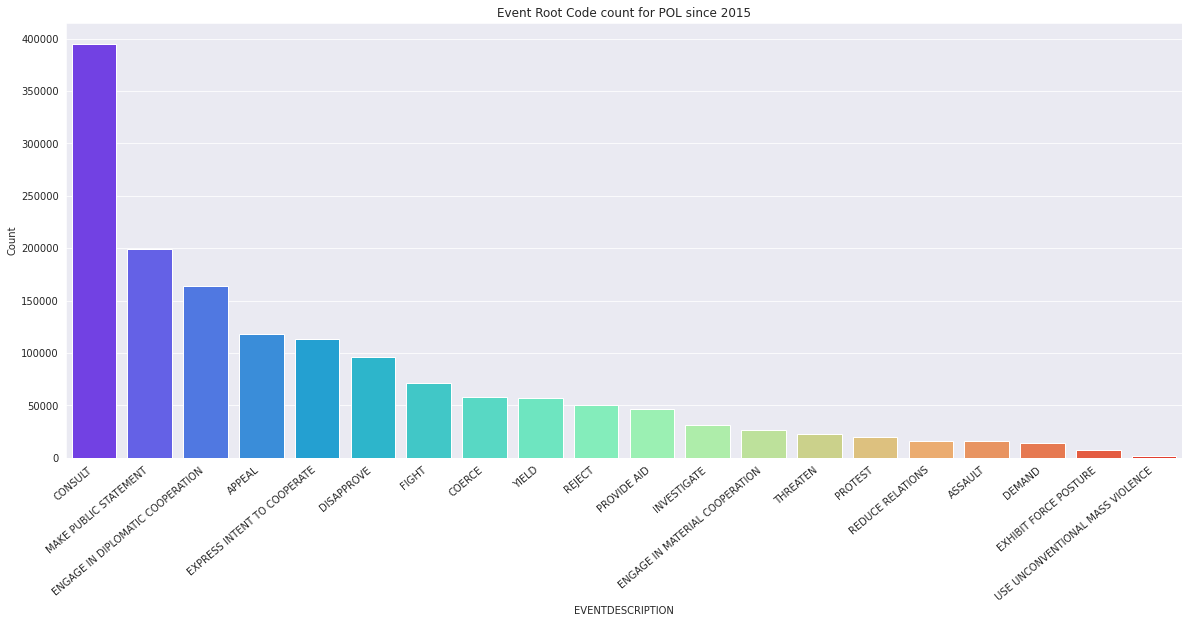
\includegraphics[width=0.8 \textwidth]{fig/PL/PLERC.png}
	\caption{Ilość zdarzeń dla poszczególnych podstawowych kodów. (zródło: opracowanie własne)}
	\label{fig:PLPERC}
	\end{figure}
		   WYKRES DO POPRAWY
 	\begin{figure}[ht]
	\centering
	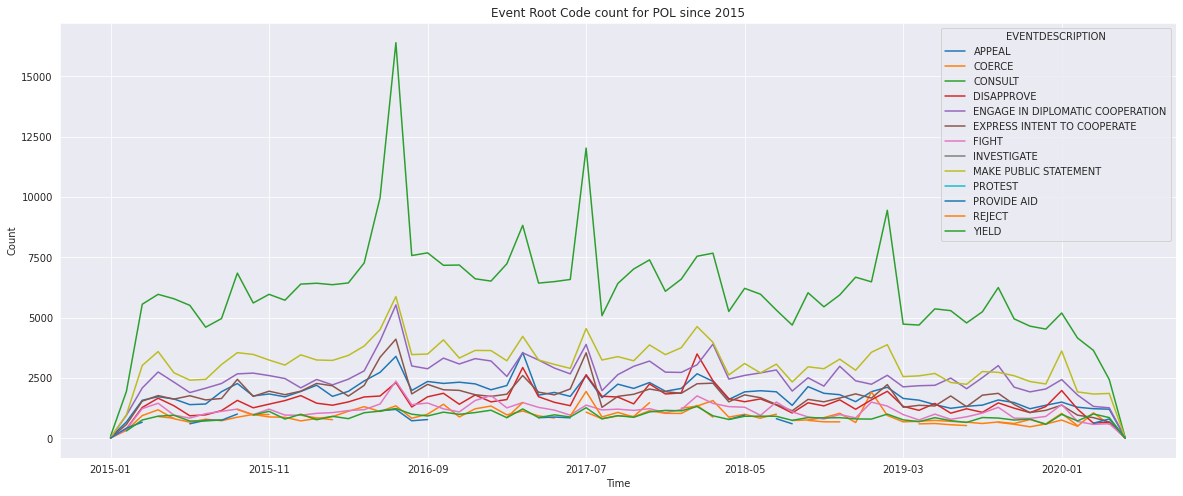
\includegraphics[width=0.8 \textwidth]{fig/PL/PLERCinTIME.png}
	\caption{Ilość zdarzeń dla poszczególnych podstawowych kodów w czasie. (zródło: opracowanie własne)}
	\label{fig:PLPERCinTIME}
	\end{figure}
 	   WYKRES DO POPRAWY
  	\begin{figure}[ht]
	\centering
	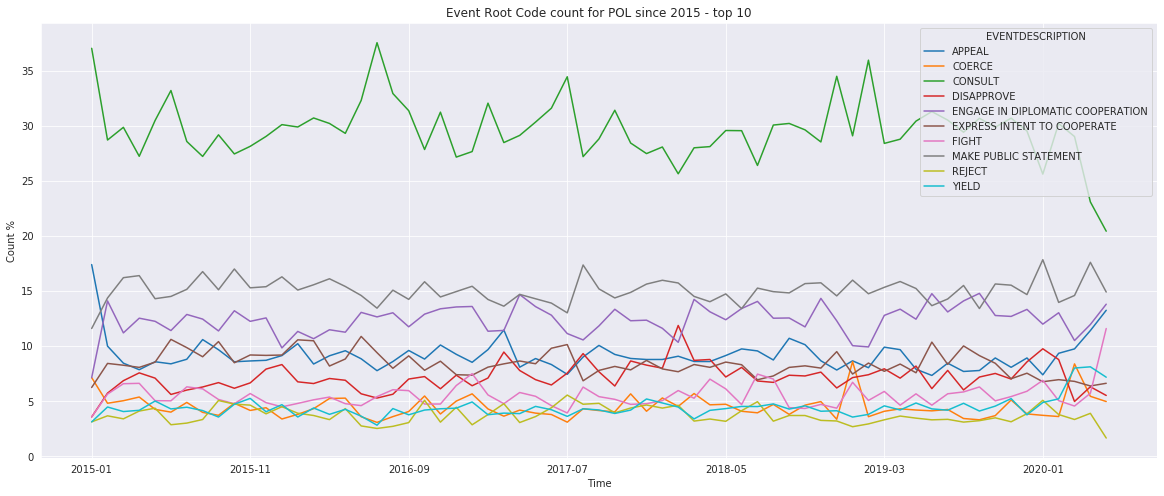
\includegraphics[width=0.8 \textwidth]{fig/PL/PLERCpercinTIME.png}
	\caption{Procentowa ilość zdarzeń dla poszczególnych podstawowych kodów w czasie. (zródło: opracowanie własne)}
	\label{fig:PLPERCpercinTIME}
	\end{figure}
	
 \subsection{Podstawowe kody zdarzeń między Polską a wybranymi krajami} 
  	   WYKRES DO POPRAWY
  	\begin{figure}[ht]
	\centering
	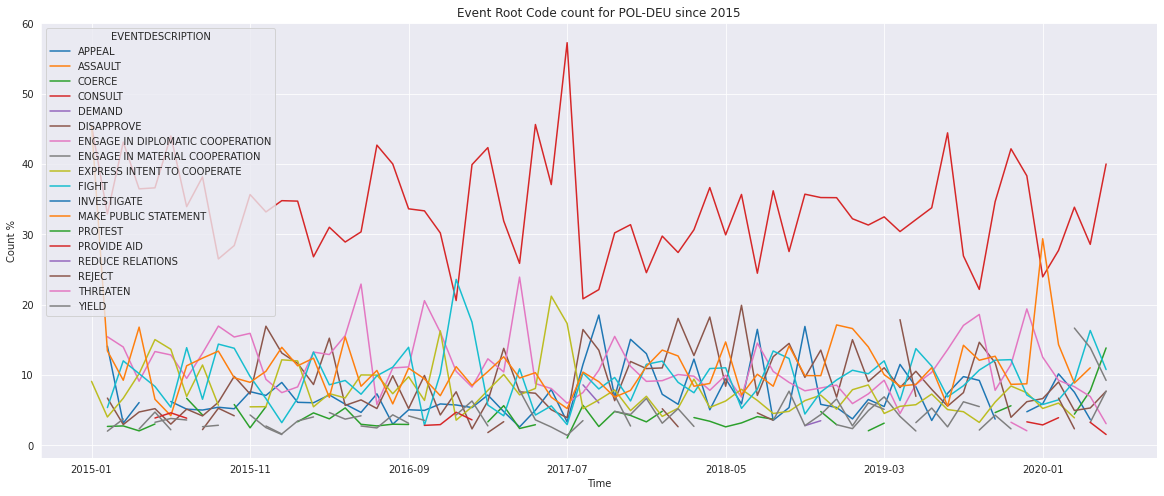
\includegraphics[width=0.8 \textwidth]{fig/PL/POLDEUERCperc.png}
	\caption{Procentowa ilość zdarzeń z Niemcami dla poszczególnych podstawowych kodów w czasie. (zródło: opracowanie własne)}
	\label{fig:PLDEUERC}
	\end{figure}
 
   	   WYKRES DO POPRAWY
  	\begin{figure}[ht]
	\centering
	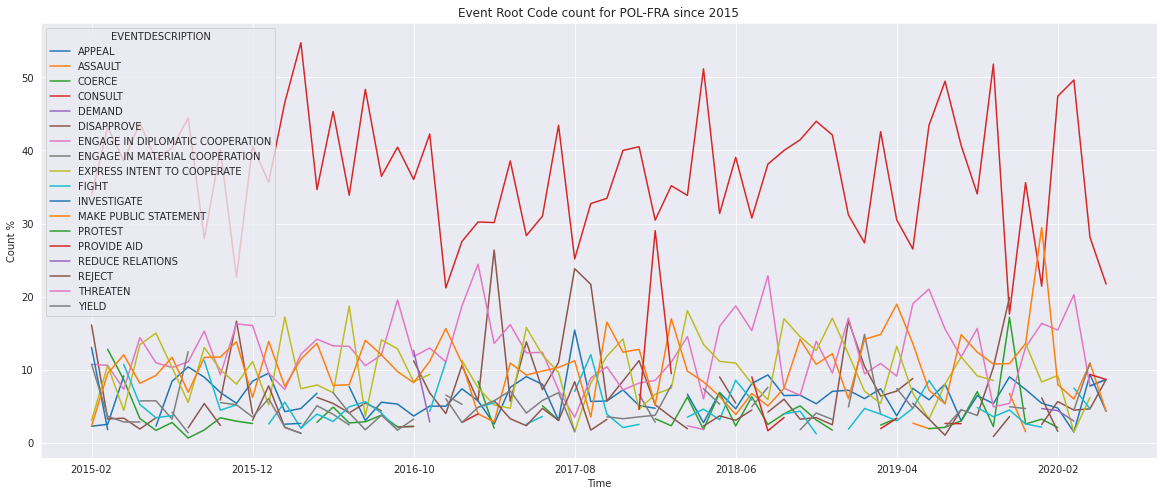
\includegraphics[width=0.8 \textwidth]{fig/PL/POLFRAERCperc.png}
	\caption{Procentowa ilość zdarzeń z Francją dla poszczególnych podstawowych kodów w czasie. (zródło: opracowanie własne)}
	\label{fig:PLFRAERC}
	\end{figure}
	
	   	   WYKRES DO POPRAWY
  	\begin{figure}[ht]
	\centering
	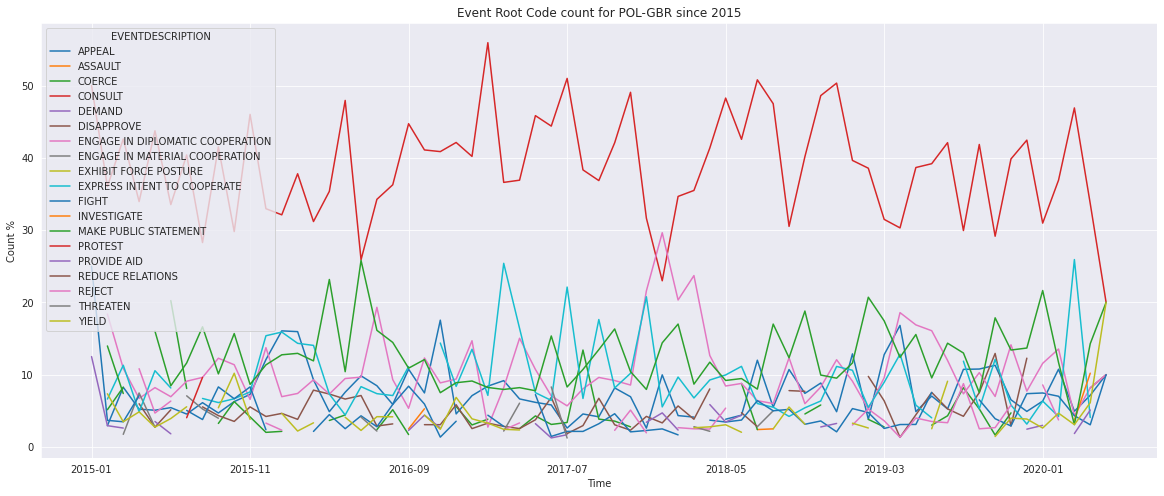
\includegraphics[width=0.8 \textwidth]{fig/PL/POLGBRERCperc.png}
	\caption{Procentowa ilość zdarzeń z Wielka Brytanią dla poszczególnych podstawowych kodów w czasie. (zródło: opracowanie własne)}
	\label{fig:PLGBRERC}
	\end{figure}
	
		   	   WYKRES DO POPRAWY
  	\begin{figure}[ht]
	\centering
	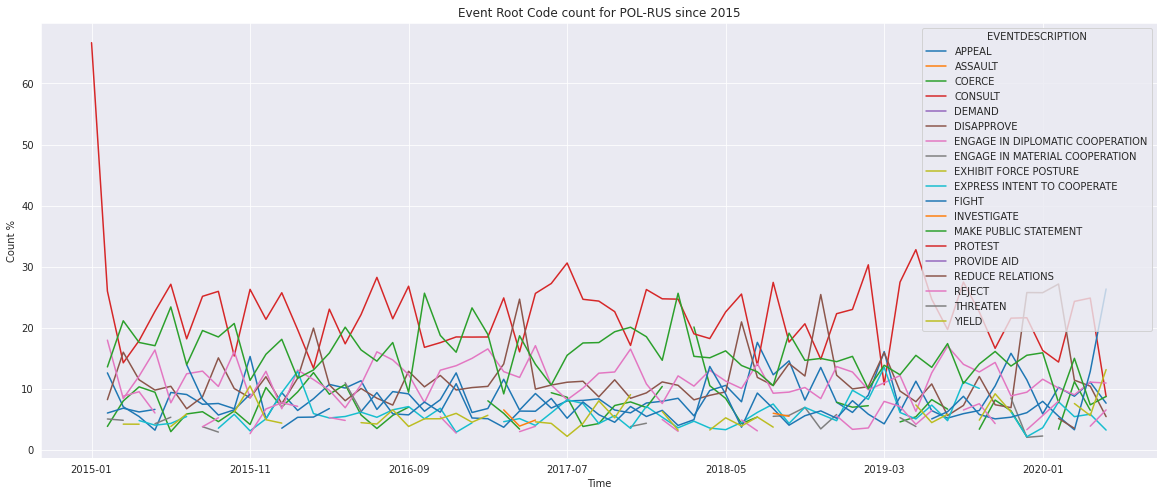
\includegraphics[width=0.8 \textwidth]{fig/PL/POLRUSERCperc.png}
	\caption{Procentowa ilość zdarzeń z Rosją dla poszczególnych podstawowych kodów w czasie. (zródło: opracowanie własne)}
	\label{fig:PLRUSERC}
	\end{figure}
	
	
	
 \section{Niemcy}
 \section{Rosja}
 \section{Stan zjednoczone}
 \section{Pozostałe}
 
 \chapter{Analiza siły powiązania}
 \section{Analiza siły powiązania miedzy wybranymi krajami}
 \subsection{Polska}

  	\begin{figure}[ht]
	\centering
	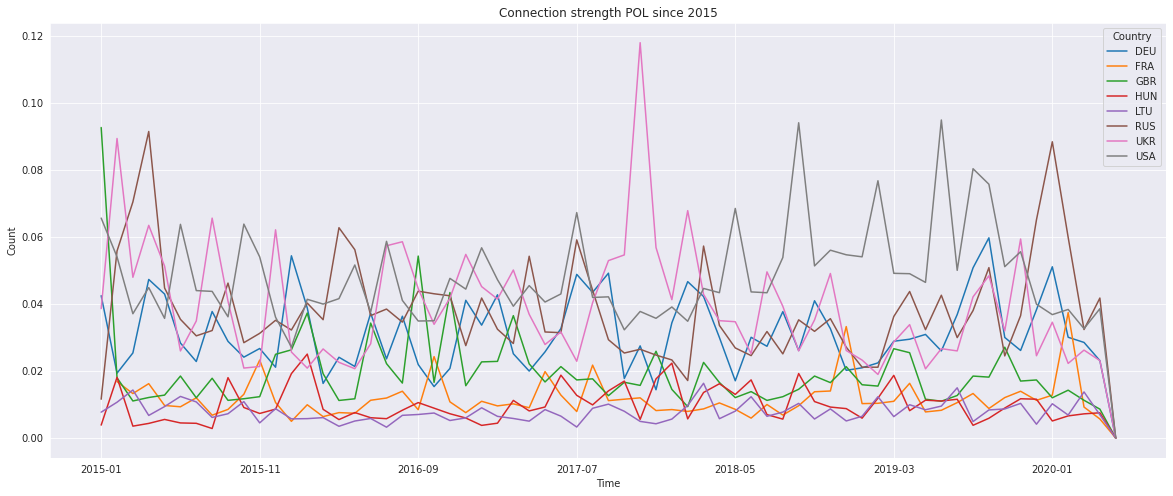
\includegraphics[width=0.8 \textwidth]{fig/PL/POLConnection.png}
	\caption{Siła połączenia Polski z wybranymi krajami w czasie. (zródło: opracowanie własne)}
	\label{fig:PLConnection}
	\end{figure}
	
 \subsection{Rosja}
 
   	\begin{figure}[ht]
	\centering
	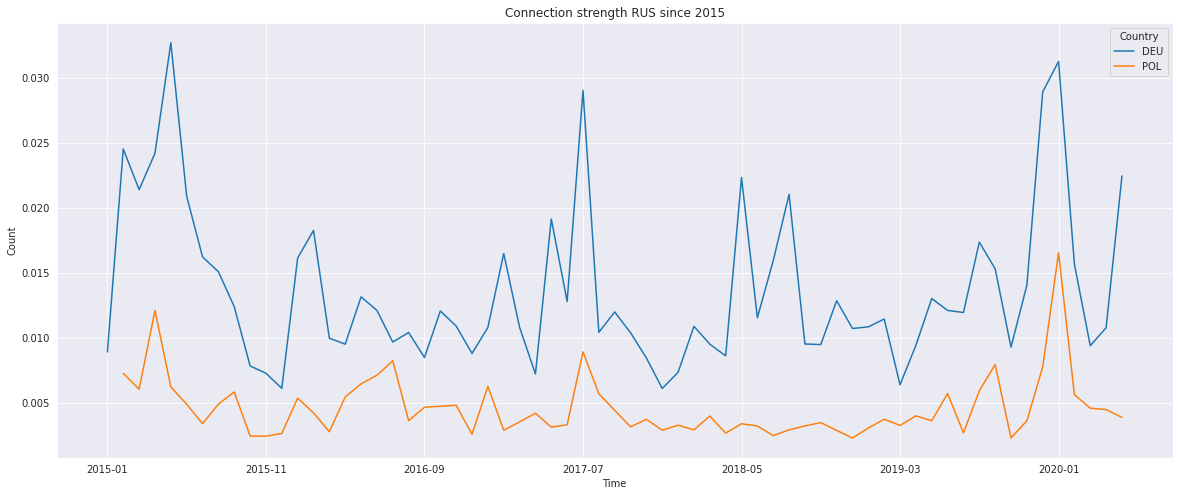
\includegraphics[width=0.8 \textwidth]{fig/RUS/RUSConnection.png}
	\caption{Siła połączenia Rosji z wybranymi krajami w czasie. (zródło: opracowanie własne)}
	\label{fig:RUSConnection}
	\end{figure}
 
 \subsection{Niemcy}
 
    \begin{figure}[ht]
	\centering
	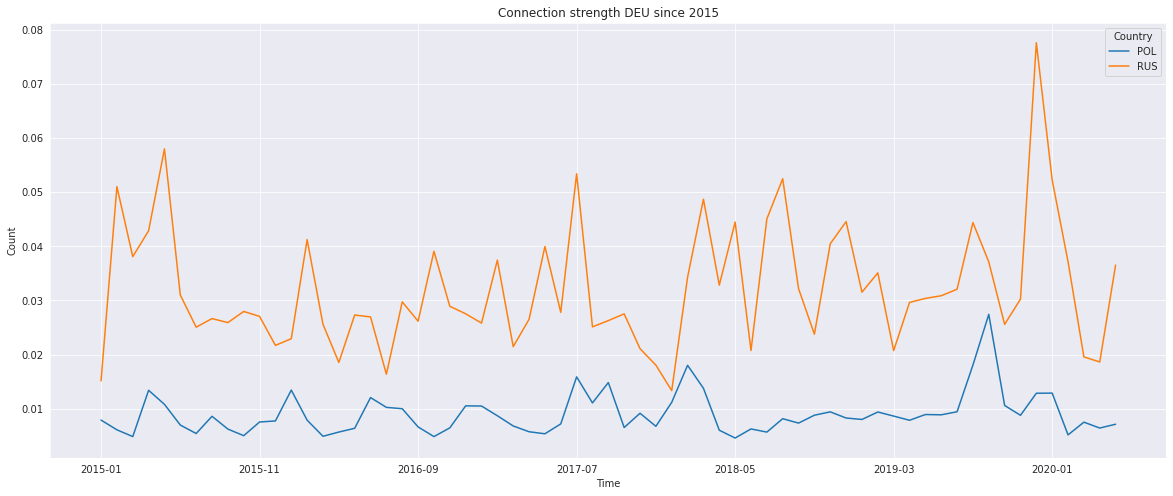
\includegraphics[width=0.8 \textwidth]{fig/DEU/DEUConnection.png}
	\caption{Siła połączenia Niemiec z wybranymi krajami w czasie. (zródło: opracowanie własne)}
	\label{fig:DEUConnection}
	\end{figure}
	
 \subsection{Stany Zjednoczone}
 
    \begin{figure}[ht]
	\centering
	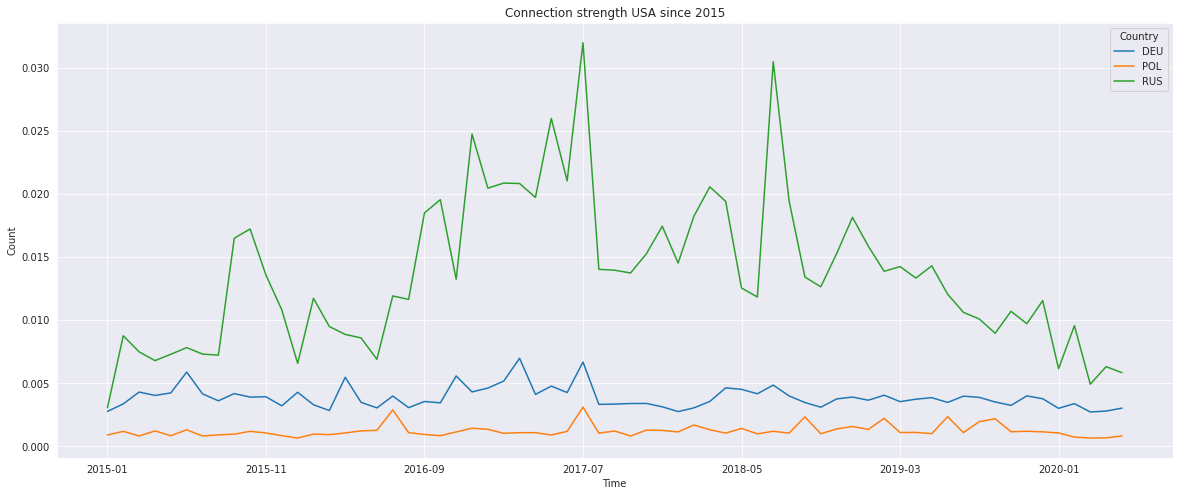
\includegraphics[width=0.8 \textwidth]{fig/USA/USAConnection.png}
	\caption{Siła połączenia Stanów Zjednoczonych z wybranymi krajami w czasie. (zródło: opracowanie własne)}
	\label{fig:USAConnection}
	\end{figure}
	
 \section{Analiza symetryczności siły powiązania}
 \subsection{Polska - Niemcy - Polska}
  
    \begin{figure}[ht]
	\centering
	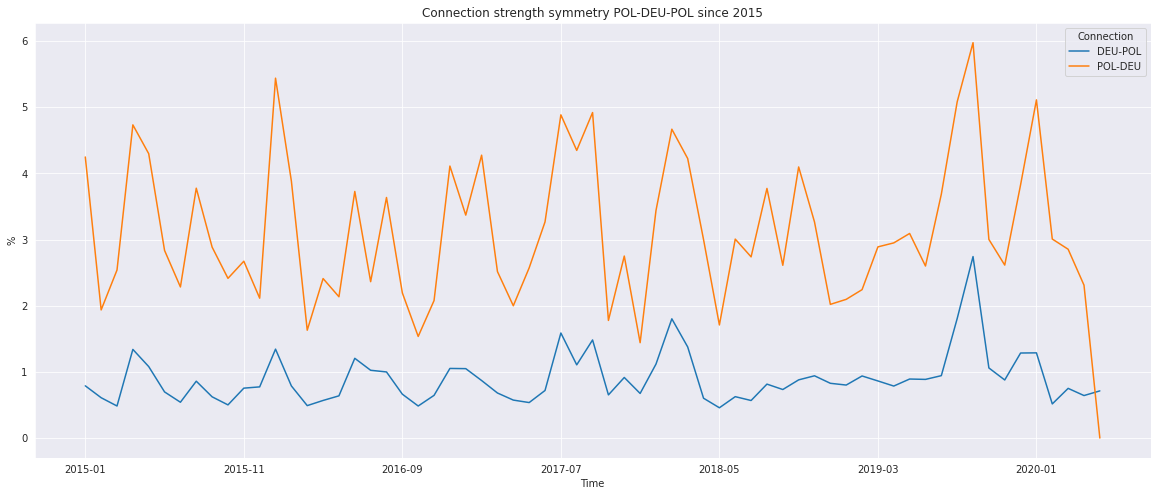
\includegraphics[width=0.8 \textwidth]{fig/ConnectionSymmetry/POL-DEU-POL.png}
	\caption{Symetryczność siły połączenia Polski i Niemiec w czasie. (zródło: opracowanie własne)}
	\label{fig:POL-DEU-POL}
	\end{figure}
	
 \subsection{Polska - Rosja - Polska}
  
    \begin{figure}[ht]
	\centering
	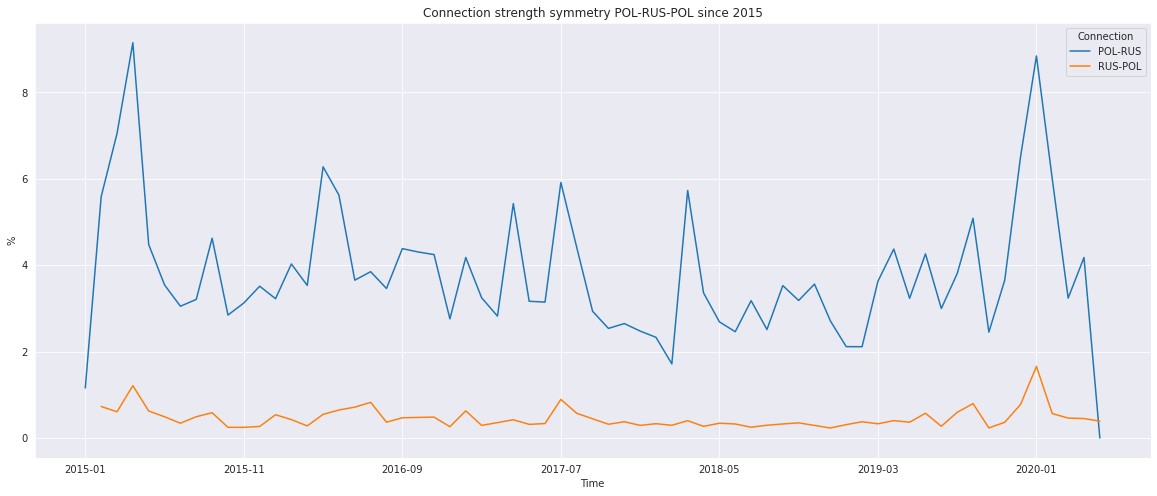
\includegraphics[width=0.8 \textwidth]{fig/ConnectionSymmetry/POL-RUS-POL.png}
	\caption{Symetryczność siły połączenia Polski i Rosji w czasie. (zródło: opracowanie własne)}
	\label{fig:POL-RUS-POL}
	\end{figure}
	
 \subsection{Polska - Stany Zjednoczone - Polska}
  
    \begin{figure}[ht]
	\centering
	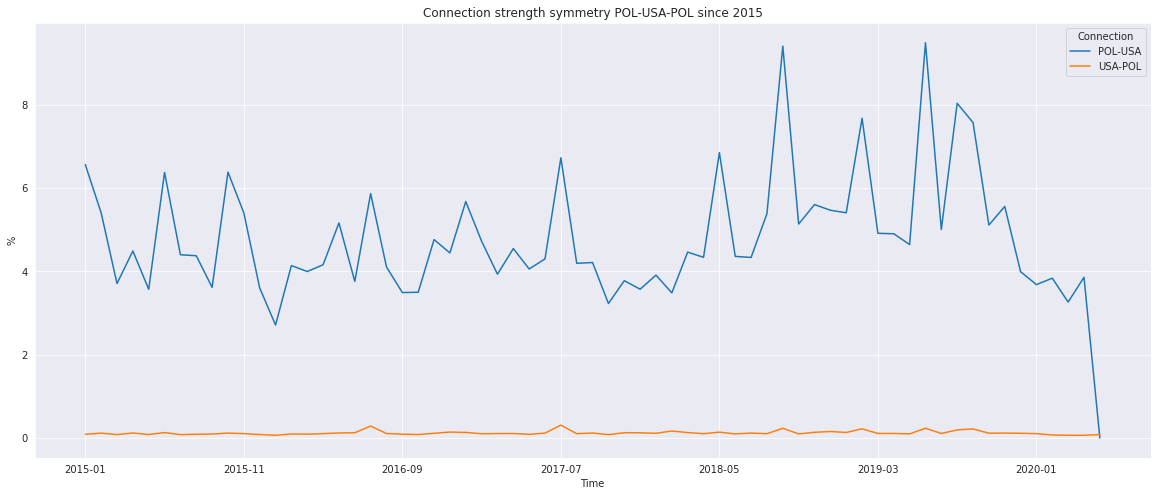
\includegraphics[width=0.8 \textwidth]{fig/ConnectionSymmetry/POL-USA-POL.png}
	\caption{Symetryczność siły połączenia Polski i Stanów Zjednoczonych w czasie. (zródło: opracowanie własne)}
	\label{fig:POL-USA-POL}
	\end{figure}
 
 
 \chapter{Klasteryzacja} 
 
 \chapter{Podsumowanie}
W niniejszej części zostaną opisane wnioski z pracy według kolejności wcześniej przedstawionych rozdziałów.


 \inputencoding{utf8}
 
 \newpage
 \addcontentsline{toc}{chapter}{Książki}
 \printbibliography[title={Książki},type=book]
 
 \addcontentsline{toc}{chapter}{Artykuły}
 \printbibliography[title={Artykuły},type=article]
 
 \addcontentsline{toc}{chapter}{Prace dyplomowe}
 \printbibliography[title={Prace dyplomowe}, type=thesis]
 
 \addcontentsline{toc}{chapter}{Materiały konferencyjne}
 \printbibliography[title={Materiały konferencyjne},type=inproceedings]
 
 \addcontentsline{toc}{chapter}{Pozostałe źródła}
 \printbibliography[title={Pozostałe źródła}, nottype=article, nottype=book, nottype=inproceedings, nottype=thesis]

 \end{document}
